\documentclass[12pt]{article}
\usepackage[paper=letterpaper,margin=2cm]{geometry}
\usepackage{amsmath,amssymb,amsfonts}
\usepackage{newtxtext, newtxmath}
\usepackage{enumitem}
\usepackage{titling}
\usepackage{nicematrix}
\usepackage[colorlinks=true]{hyperref}
\usepackage{graphicx}
\usepackage{listings}
\usepackage{mathtools}

\setlength{\droptitle}{-6em}

\DeclareMathOperator*{\argmax}{arg\,max}

\begin{document}

\newcommand{\prob}{\textrm{P}}
\newcommand{\ind}{\perp\!\!\!\!\!\perp} 
\newcommand{\notind}{\not\perp\!\!\!\!\!\perp}
\newcommand{\defeq}{\vcentcolon=}

\center
Aprendizagem 2023\\
Homework II -- Group 016\\
(ist1100293, ist1102556)\vskip 1cm

\large{\textbf{Part I}: Pen and paper}\normalsize

\begin{enumerate}[leftmargin=\labelsep]

\item Consider $\mathbf{x}_1$-$\mathbf{x}_7$ to be training observations, $\mathbf{x}_8$-$\mathbf{x}_9$ to be testing observations, $y_1$-$y_5$ to be input
variables and $y_6$ to be the target variable.
Hint: you can use scipy.stats.multivariate\_normal for multivariate distribution calculus

    We used the following code to get the values of the multivariate normal PDF's:

    \begin{center}
        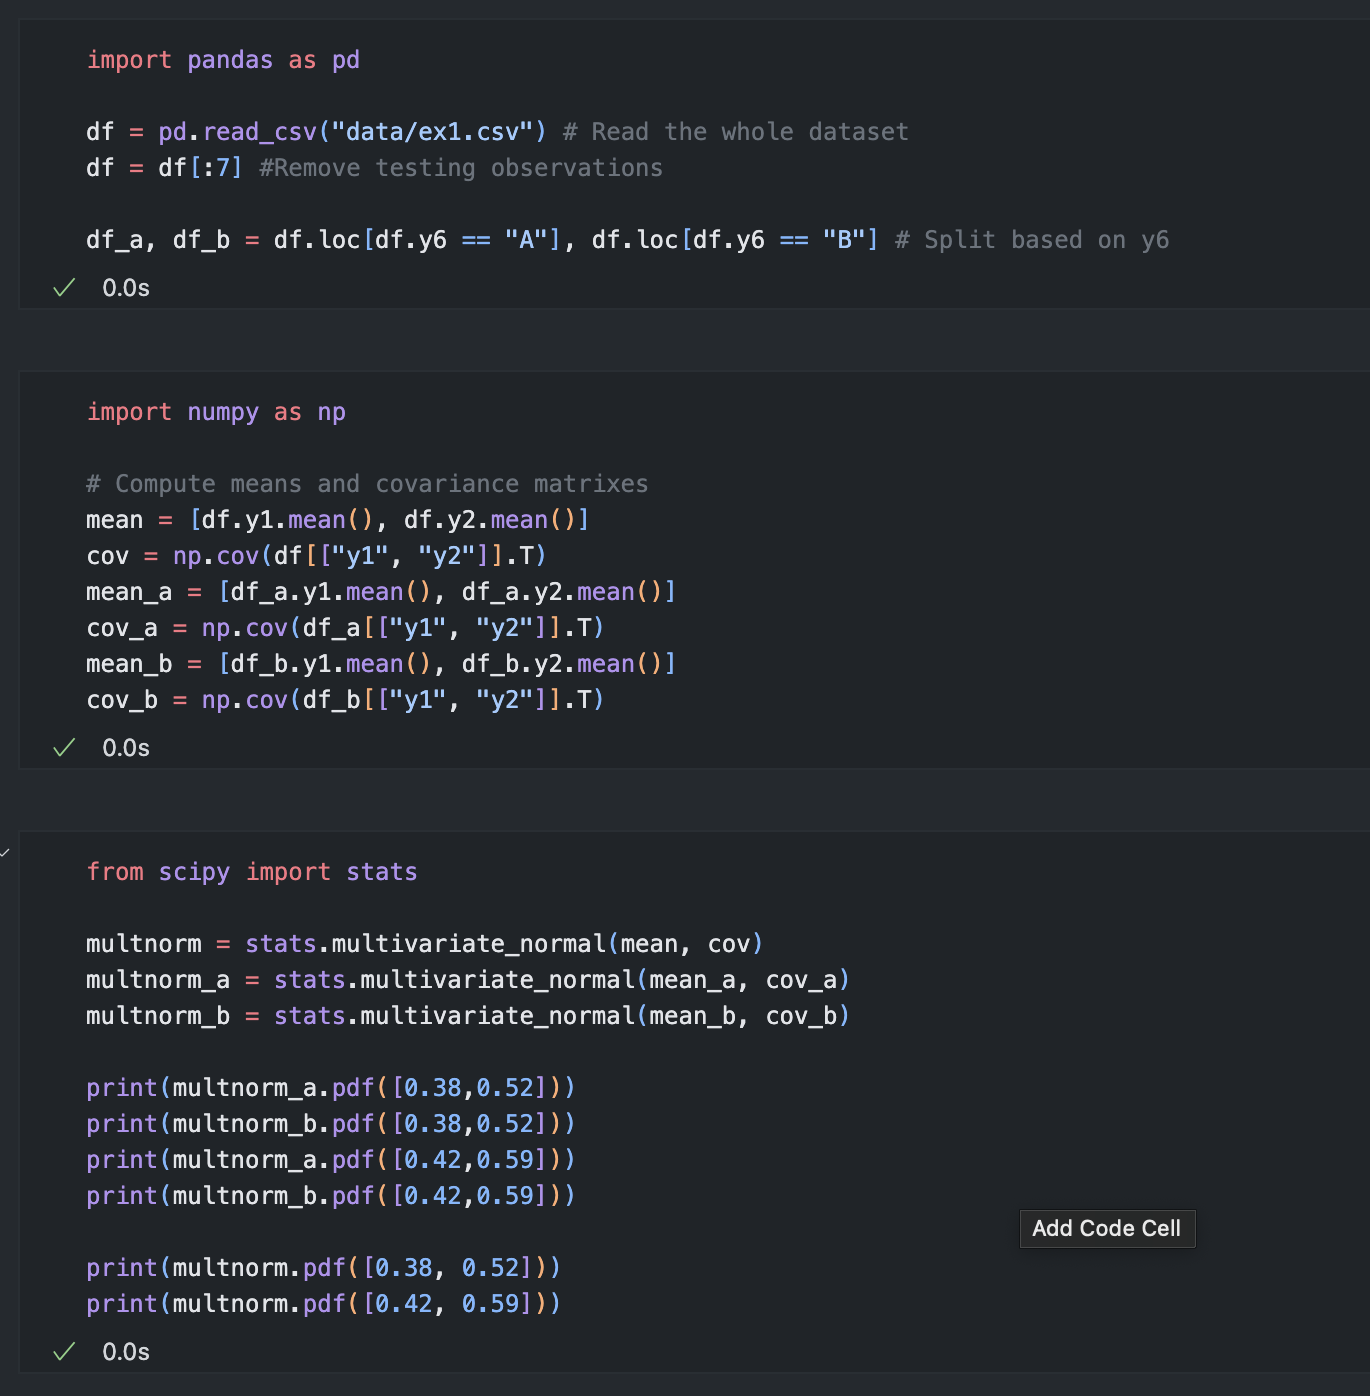
\includegraphics[scale=0.5]{images/code1.png}
    \end{center}

    \begin{enumerate}
        \item Learn a Bayesian classifier assuming: i) ${y_1, y_2}$, ${y_3, y_4}$ and ${y_5}$ sets of independent
        variables (e.g., $y_1 \ind y_3$ yet $y_1 \notind y_2$), and ii) $y_1 \times y_2 \in \mathbb{R}^2$
        is normally distributed. Show all
        parameters (distributions and priors for subsequent testing).

        \paragraph{} Since the variables $y_1$-$y_5$ can be divided into the independent subsets: $\{y_1, y_2\}, \{y_3, y_4\}, \{y_5\}$, we have:

        \begin{multline}
            \prob(y_1 = x_1, y_2 = x_2, y_3 = x_3, y_4 = x_4, y_5 = x_5 | y_6 = C) = \\
            \prob(y_1 = x_1, y_2 = x_2 | y_6 = C)\prob(y_3 = x_3, y_4 = x_4|y_6 = C)\prob(y_5 = x_5|y_6 = C)
        \end{multline}

        \paragraph{Priors}
        \begin{equation}
            \prob(y_6 = A) = \frac{3}{7} \qquad \prob(y_6 = B) = \frac{4}{7}
        \end{equation}

        \paragraph{Y1 and Y2 Conditional PDF's}
        Since we are assuming that $y_1$ and $y_2$ are normally distributed, we will replace the conditional probabilities of $y_1$ and $y_2$ with the value of the conditional PDF of these variables.

        \begin{equation}
        \begin{split}
            \prob(y_1 = x_1, y_2 = x_2 | y_6 = C) &\defeq \textrm{N}(\mathbf{x} | \mu_C, \Sigma_C) \\
            &\defeq \frac{1}{(2\pi)^{m/2}\sqrt{|\Sigma_C|}}\exp\Bigl(-\frac{1}{2}(\mathbf{x}-\mu_C)^\intercal \Sigma_C^{-1} (\mathbf{x}-\mu_C)\Bigr)
        \end{split}
        \end{equation}

        Where $\mu_C$ is the class conditional multivariate average of the data,

        \begin{equation}
        \mu_A = \begin{bmatrix}
            \frac{0.24 + 0.16 + 0.32}{3} \\
            \frac{0.36 + 0.48 + 0.72}{3}
        \end{bmatrix} = \begin{bmatrix}
            0.24 \\
            0.52
        \end{bmatrix}
        \end{equation}

        \begin{equation}
            \mu_B =
            \begin{bmatrix}
                \frac{0.54 + 0.66 + 0.76 + 0.41}{4} \\
                \frac{0.11 + 0.39 + 0.28 + 0.53}{4}
            \end{bmatrix} =
            \begin{bmatrix}
                0.5925 \\
                0.3275
            \end{bmatrix}
        \end{equation}

        and $\Sigma_C$ is the class conditional covariance matrix of the data:

        \begin{equation}
            \Sigma_C =
            \begin{bmatrix}
                \textrm{var}(y_1)_C & \textrm{cov}(y_1, y_2)_C \\
                \textrm{cov}(y_1)_C & \textrm{var}(y_2)_C
            \end{bmatrix} 
        \end{equation}

        Where $\textrm{var}(y) = \frac{1}{N-1}\sum_{i = 0}^{N}(x_i - \bar{y})^2$ and $\textrm{cov}(y_1, y_2) = \frac{1}{N-1}\sum_{i = 0}^{N}(x_{1i} - \bar{y_1})(x_{2i} - \bar{y_2})$.
        So we have:

        \begin{equation}
        \begin{split}
            \textrm{var}(y_1)_A &= \frac{(0.24-0.24)^2 + (0.16-0.24)^2 + (0.32-0.24)^2}{2} = 0.0064 \\
            \textrm{var}(y_2)_A &= \frac{(0.36-0.52)^2 + (0.48-0.52)^2 + (0.72-0.52)^2}{2} = 0.0336 \\
            \textrm{cov}(y_1, y_2)_A &= \frac{(0.24-0.24)(0.36-0.52) + (0.16-0.24)(0.48-0.52)}{2}+ \\
            &+ \frac{(0.32-0.24)(0.72-0.52)}{2} = 0.0096
        \end{split}
        \end{equation}

        \begin{equation}
            \Sigma_A =
            \begin{bmatrix}
                \textrm{var}(y_1)_A & \textrm{cov}(y_1, y_2)_A \\
                \textrm{cov}(y_1)_A & \textrm{var}(y_2)_A
            \end{bmatrix}=
            \begin{bmatrix}
                0.0064 & 0.0096 \\
                0.0096 & 0.0363
            \end{bmatrix}
        \end{equation}

        \begin{equation}
            \Sigma_B =
            \begin{bmatrix}
                \textrm{var}(y_1)_B & \textrm{cov}(y_1, y_2)_B \\
                \textrm{cov}(y_1)_B & \textrm{var}(y_2)_B
            \end{bmatrix}=
            \begin{bmatrix}
                0.0229 & -0.0098 \\
                -0.0098 & 0.0315
            \end{bmatrix}
        \end{equation}

        \paragraph{Y3 and Y4 Conditional PMF's}

        \begin{equation}
        \begin{split}
            \prob(y_3 = 0, y_4 = 0 | y_6 = A) = 0 &\qquad \prob(y_3 = 0, y_4 = 0 | y_6 = B) = \frac{1}{2} \\
            \prob(y_3 = 0, y_4 = 1 | y_6 = A) = \frac{1}{3} &\qquad \prob(y_3 = 0, y_4 = 1 | y_6 = B) = \frac{1}{4} \\
            \prob(y_3 = 1, y_4 = 0 | y_6 = A) = \frac{1}{3} &\qquad \prob(y_3 = 1, y_4 = 0 | y_6 = B) = \frac{1}{4} \\
            \prob(y_3 = 1, y_4 = 1 | y_6 = A) = \frac{1}{3} &\qquad \prob(y_3 = 1, y_4 = 1 | y_6 = B) = 0
        \end{split}
        \end{equation}

        \paragraph{Y5 Conditional PMF's}

        \begin{equation}
        \begin{split}
            \prob(y_5 = 0 | y_6 = A) = \frac{1}{3} &\qquad \prob(y_5 = 0 | y_6 = B) = \frac{1}{4} \\
            \prob(y_5 = 1 | y_6 = A) = \frac{1}{3} &\qquad \prob(y_5 = 1 | y_6 = B) = \frac{1}{2} \\
            \prob(y_5 = 2 | y_6 = A) = \frac{1}{3} &\qquad \prob(y_5 = 2 | y_6 = B) = \frac{1}{4}
        \end{split}
        \end{equation}

        \paragraph{Whole Probabilities}

        (Even though you don't need the values of the whole probabilities (evidences) to classify according to MAP o ML, we will still compute those in case we need later.)

        \begin{equation}
            \prob(y_1 = x_1, y_2 = x_2) = \textrm{N}(\mathbf{x} | \mu, \Sigma)
        \end{equation}

        Where:
    
        \begin{equation}
            \mu = \begin{bmatrix}
                0.4414 \\
                0.4100
            \end{bmatrix} \qquad \Sigma = \begin{bmatrix}
                0.0491 & -0.0211 \\
                -0.0211 & 0.0375
            \end{bmatrix}
        \end{equation}

        \begin{equation}
        \begin{split}
            \prob(y_3 = 0, y_4 = 0) = \frac{2}{7} &\qquad \prob(y_3 = 0, y_4 = 1) = \frac{2}{7} \\
            \prob(y_3 = 1, y_4 = 0) = \frac{2}{7} &\qquad \prob(y_3 = 1, y_4 = 1) = \frac{1}{7}
        \end{split}
        \end{equation}

        \begin{equation}
            \prob(y_5 = 0) = \frac{2}{7} \qquad \prob(y_5 = 1) = \frac{3}{7} \qquad \prob(y_5 = 2) = \frac{2}{7}
        \end{equation}

        \item Under a MAP assumption, classify each testing observation showing all your calculus.
    
        \begin{equation}
            \textrm{MAP}(\textbf{x}) = \argmax_C \frac{\prob(\textbf{x}|y_6 = C)\prob(y_6 = C)}{\prob(\textbf{x})}
        \end{equation}

        Since $\prob(\textbf{x})$ is independent of $C$, we have:

        \begin{equation}
            \textrm{MAP}(\textbf{x}) = \argmax_C \prob(\textbf{x}|y_6 = C)\prob(y_6 = C)
        \end{equation}

        \paragraph{For x8:}

        \begin{equation}
        \begin{split}
            \prob(y_1 = 0.38, y_2 = 0.52, y_3 = 0, y_4 = 1, y_5 = 0|y_6 = A)\prob(y_6 = A)\\
            = \prob(y_1 = 0.38, y_2 = 0.52|y_6 = A)\prob(y_3 = 0, y_4 = 1|y_6 = A)\prob(y_5 = 0|y_6 = A)\prob(y_6 = A)\\
            \approx 0.9847 \times \frac{1}{3} \times \frac{1}{3} \times \frac{3}{7} \approx 0.04689
        \end{split}
        \end{equation}

        \begin{equation}
        \begin{split}
            \prob(y_1 = 0.38, y_2 = 0.52, y_3 = 0, y_4 = 1, y_5 = 0|y_6 = B)\prob(y_6 = B)\\
            = \prob(y_1 = 0.38, y_2 = 0.52|y_6 = B)\prob(y_3 = 0, y_4 = 1|y_6 = B)\prob(y_5 = 0|y_6 = B)\prob(y_6 = B)\\
            \approx 1.9624 \times \frac{1}{4} \times \frac{1}{4} \times \frac{4}{7} \approx 0.07009
        \end{split}
        \end{equation}

        According to a MAP assumption, we classify $\mathbf{x}_8$ as $\hat{y}_6 = B$.

        \paragraph{For x9:}

        \begin{equation}
        \begin{split}
            \prob(y_1 = 0.42, y_2 = 0.59, y_3 = 0, y_4 = 1, y_5 = 1|y_6 = A)\prob(y_6 = A)\\
            = \prob(y_1 = 0.42, y_2 = 0.59|y_6 = A)\prob(y_3 = 0, y_4 = 1|y_6 = A)\prob(y_5 = 1|y_6 = A)\prob(y_6 = A)\\
            \approx 0.4031 \times \frac{1}{3} \times \frac{1}{3} \times \frac{3}{7} \approx 0.0192
        \end{split}
        \end{equation}

        \begin{equation}
        \begin{split}
            \prob(y_1 = 0.42, y_2 = 0.59, y_3 = 0, y_4 = 1, y_5 = 1|y_6 = B)\prob(y_6 = B)\\
            = \prob(y_1 = 0.42, y_2 = 0.59|y_6 = B)\prob(y_3 = 0, y_4 = 1|y_6 = B)\prob(y_5 = 1|y_6 = B)\prob(y_6 = B)\\
            \approx 1.7286 \times \frac{1}{4} \times \frac{1}{2} \times \frac{4}{7} \approx 0.1235
        \end{split}
        \end{equation}

        According to a MAP assumption, we classify $\mathbf{x}_9$ as $\hat{y}_6 = B$.

        \item  Consider that the default decision threshold of $\theta = 0.5$ can be adjusted according to
    
            \[ 
            f(\mathbf{x}|\theta)= \left\{
            \begin{array}{ll}
                  \textrm{A} & \prob(\textrm{A}|\mathbf{x}) > \theta \\
                  \textrm{B} & \textrm{otherwise}
            \end{array} 
            \right. 
            \]

            Under a maximum likelihood assumption, what thresholds optimize testing accuracy?

            \begin{equation}
                \textrm{ML}(\mathbf{x}) = \argmax_C \prob(\mathbf{x}|y_6 = C)
            \end{equation}

            \paragraph{ML prediction for x8}

            \begin{equation}
            \begin{split}
                \prob(y_1 = 0.38, y_2 = 0.52, y_3 = 0, y_4 = 1, y_5 = 0|y_6 = A) \\
                = \prob(y_1 = 0.38, y_2 = 0.52|y_6 = A)\prob(y_3 = 0, y_4 = 1|y_6 = A)\prob(y_5 = 0|y_6 = A) \\
                \approx 0.9847 \times \frac{1}{3} \times \frac{1}{3} \approx 0.1094
            \end{split}
            \end{equation}

            \begin{equation}
            \begin{split}
                \prob(y_1 = 0.38, y_2 = 0.52, y_3 = 0, y_4 = 1, y_5 = 0|y_6 = B) \\
                = \prob(y_1 = 0.38, y_2 = 0.52|y_6 = B)\prob(y_3 = 0, y_4 = 1|y_6 = B)\prob(y_5 = 0|y_6 = B) \\
                \approx 1.9624 \times \frac{1}{4} \times \frac{1}{4} \approx 0.1227
            \end{split}
            \end{equation}

            \paragraph{ML prediction for x9}

            \begin{equation}
            \begin{split}
                \prob(y_1 = 0.42, y_2 = 0.59, y_3 = 0, y_4 = 1, y_5 = 1|y_6 = A) \\
                = \prob(y_1 = 0.42, y_2 = 0.59|y_6 = A)\prob(y_3 = 0, y_4 = 1|y_6 = A)\prob(y_5 = 1|y_6 = A) \\
                \approx 0.4031 \times \frac{1}{3} \times \frac{1}{3} \approx 0.0448
            \end{split}
            \end{equation}

            \begin{equation}
            \begin{split}
                \prob(y_1 = 0.42, y_2 = 0.59, y_3 = 0, y_4 = 1, y_5 = 1|y_6 = B) \\
                = \prob(y_1 = 0.42, y_2 = 0.59|y_6 = B)\prob(y_3 = 0, y_4 = 1|y_6 = B)\prob(y_5 = 1|y_6 = B) \\
                \approx 1.7286 \times \frac{1}{4} \times \frac{1}{2} \approx 0.2161
            \end{split}
            \end{equation}

            Under a maximum likelihood assumption, both $\mathbf{x}_8$ and $\mathbf{x}_9$ get classified as $\hat{y}_6 = B$.

            Since we are using the values of PDF's when computing the values of the likelihoods and consequently the posteriors, we need to normalize these values. Since the first are not truly probabilities (by the mathematical definition), we will denote them by $\prob^*(\mathbf{x})$ while true (normalized) probabilities will be denoted by $\prob(\mathbf{x})$.
            Since we are assuming that the classes are uniformly distributed, the prior probability will be equal for both classes. That way, both the prior and the whole probability for the features will be constants, and will not matter after normalization.
            
            \begin{equation}
            \begin{split}
                \prob(A|\mathbf{x}) &= \frac{\prob^*(A|\mathbf{x})}{\prob^*(A|\mathbf{x}) + \prob^*(B|\mathbf{x})} = \frac{\frac{\prob^*(\mathbf{x}|A)\prob(A)}{\prob^*(\mathbf{x})}}{\frac{\prob^*(\mathbf{x}|A)\prob(A)}{\prob^*(\mathbf{x})} + \frac{\prob^*(\mathbf{x}|B)\prob(B)}{\prob^*(\mathbf{x})}} \\
                &= \frac{\prob^*(\mathbf{x}|A)\cdot\frac{1}{2}}{\prob^*(\mathbf{x}|A)\cdot\frac{1}{2} + \prob^*(\mathbf{x}|B)\cdot\frac{1}{2}} = \frac{\prob^*(\mathbf{x}|A)}{\prob^*(\mathbf{x}|A) + \prob^*(\mathbf{x}|B)}
            \end{split}
            \end{equation}

            So, we have:
            
            \begin{equation}
            \begin{split}
                \prob^*(y_6 = A | \mathbf{x}_8) &\propto \prob^*(\mathbf{x}_8 | y_6 = A) \approx 0.1094 \\
                \prob^*(y_6 = B | \mathbf{x}_8) &\propto \prob^*(\mathbf{x}_8 | y_6 = B) \approx 0.1227 \\
                \prob^*(y_6 = A | \mathbf{x}_9) &\propto \prob^*(\mathbf{x}_9 | y_6 = A) \approx 0.0448 \\
                \prob^*(y_6 = B | \mathbf{x}_9) &\propto \prob^*(\mathbf{x}_9 | y_6 = B) \approx 0.2161
            \end{split}
            \end{equation}

            \paragraph{Normalizing:}

            \begin{equation}
            \begin{split}
                \prob(y_6 = A | \mathbf{x}_8) &= \frac{\prob^*(y_6 = A | \mathbf{x}_8)}{\prob^*(y_6 = A | \mathbf{x}_8) + \prob^*(y_6 = B | \mathbf{x}_8)} \approx \frac{0.1094}{0.1094 + 0.1227} \approx 0.4713 \\
                \prob(y_6 = A | \mathbf{x}_9) &\approx \frac{0.0448}{0.0448 + 0.2161} \approx 0.1717
            \end{split}
            \end{equation}

            Since the ML assumption classifies $\mathbf{x}_8$ and $\mathbf{x}_9$ as $\hat{y}_6 = B$, we need to find a threshold that makes the new classifier agree with the ML assumption (to maximize the accuracy) for the testing dataset.
            We can choose $\theta \geq 0.4713$ since with those values, both of the posterior probabilities for the class A will be lower or equal than that, and the classifier will output $\hat{y}_6 = B$.

    \end{enumerate}

    \item Let $y_1$ be the target numeric variable, $y_2$-$y_6$ be the input variables where $y_2$ is binarized under an
    equal-width (equal-range) discretization. For the evaluation of regressors, consider a 3-fold
    cross-validation over the full dataset ($\mathbf{x}_1$-$\mathbf{x}_9$) without shuffling the observations.

    \begin{enumerate}
        \item Identify the observations and features per data fold after the binarization procedure.
        
        Since it's assumed that $y_2 \in [0, 1]$ our binarization criteria will be:

        \[ 
            y_2^{\textrm{new}} = \left\{
            \begin{array}{ll}
                  0, & \textrm{if } y_2 \leq 0.5 \\
                  1, & \textrm{if } y_2 > 0.5
            \end{array} 
            \right. 
        \]

        After applying the binarization, our data is:

        \begin{center}
        \begin{tabular}{|c|c|c|c|c|c|c|}
        \hline
        D     & $y_1$ & $y_2$ & $y_3$ & $y_4$ & $y_5$ & $y_6$ \\
        \hline
        $x_1$ & 0.24  & 0     & 1     & 1     & 0     & A \\
        $x_2$ & 0.16  & 0     & 1     & 0     & 1     & A \\
        $x_3$ & 0.32  & 1     & 0     & 1     & 2     & A \\
        $x_4$ & 0.54  & 0     & 0     & 0     & 1     & B \\
        $x_5$ & 0.66  & 0     & 0     & 0     & 0     & B \\
        $x_6$ & 0.76  & 0     & 1     & 0     & 2     & B \\
        $x_7$ & 0.41  & 1     & 0     & 1     & 1     & B \\
        $x_8$ & 0.38  & 1     & 0     & 1     & 0     & A \\
        $x_9$ & 0.42  & 1     & 0     & 1     & 1     & B \\
        \hline
        \end{tabular}
        \end{center}

        \paragraph{1st fold:} Training: $\{x_1, x_2, x_3, x_4, x_5, x_6\}$ Testing: $\{x_7, x_8, x_9\}$
        \paragraph{2nd fold:} Training: $\{x_1, x_2, x_3, x_7, x_8, x_9\}$ Testing: $\{x_4, x_5, x_6\}$
        \paragraph{3rd fold:} Training: $\{x_4, x_5, x_6, x_7, x_8, x_9\}$ Testing: $\{x_1, x_2, x_3\}$
        \item  Consider a distance-weighted $k$NN with $k = 3$, Hamming distance ($d$), and $1/d$ weighting.
        Compute the MAE of this $k$NN regressor for the 1st iteration of the cross-validation (i.e. train
        observations have the lower indices).
        
        \begin{center}
            \begin{tabular}{|c|c|c|c|c|c|c|}
                \hline
                d & $x_1$ & $x_2$ & $x_3$ & $x_4$ & $x_5$ & $x_6$ \\
                \hline
                $x_7$ & 4 & 4 & \textbf{2} & \textbf{2} & \textbf{3} & 4 \\
                \hline
                $x_8$ & \textbf{2} & 4 & \textbf{1} & 4 & \textbf{3} & 5 \\
                \hline
                $x_9$ & 4 & 4 & \textbf{2} & \textbf{2} & \textbf{3} & 4 \\
                \hline
            \end{tabular}
        \end{center}

        \paragraph{For x7:}

        \begin{equation}
        \begin{split}
            k\textrm{NN}_{k = 3}(\mathbf{x}_7) = \Bigl\{ \mathbf{x}_3, \mathbf{x}_4, \mathbf{x}_5\Bigr\} \\
            w_3 = \frac{1}{2} \qquad w_4 = \frac{1}{2} \qquad w_5 = \frac{1}{3}
        \end{split}
        \end{equation}

        \begin{equation}
        \begin{split}
            \hat{y}_1(\mathbf{x}_7) &= \textrm{AverageMean}\Bigl\{ y_1(\mathbf{x}_3), y_1(\mathbf{x}_4), y_1(\mathbf{x}_5) \Bigr\} \\
            &= \frac{w_3y_1(\mathbf{x}_3) + w_4y_1(\mathbf{x}_4) + w_5y_1(\mathbf{x}_5)}{w_3 + w_4 + w_5} \\
            &= \frac{\frac{1}{2} \times 0.32 + \frac{1}{2} \times 0.54 + \frac{1}{3} \times 0.66}{\frac{1}{2} + \frac{1}{2} + \frac{1}{3}} \\
            &= 0.4875
        \end{split}
        \end{equation}

        \paragraph{For x8:}

        \begin{equation}
        \begin{split}
            k\textrm{NN}_{k = 3}(\mathbf{x}_8) = \Bigl\{ \mathbf{x}_1, \mathbf{x}_3, \mathbf{x}_5\Bigr\} \\
            w_1 = \frac{1}{2} \qquad w_3 = 1 \qquad w_5 = \frac{1}{3}
        \end{split}
        \end{equation}

        \begin{equation}
        \begin{split}
            \hat{y}_1(\mathbf{x}_8) &= \frac{w_1y_1(\mathbf{x}_1) + w_3y_1(\mathbf{x}_3) + w_5y_1(\mathbf{x}_5)}{w_1 + w_3 + w_5} \\
            &= \frac{\frac{1}{2} \times 0.24 + 1 \times 0.32 + \frac{1}{3} \times 0.66}{\frac{1}{2} + 1 + \frac{1}{3}} \\
            &= 0.36
        \end{split}
        \end{equation}

        \paragraph{For x9:}

        \begin{equation}
        \begin{split}
            k\textrm{NN}_{k = 3}(\mathbf{x}_9) = \Bigl\{ \mathbf{x}_3, \mathbf{x}_4, \mathbf{x}_5\Bigr\} \\
            w_3 = \frac{1}{2} \qquad w_4 = \frac{1}{2} \qquad w_5 = \frac{1}{3}
        \end{split}
        \end{equation}

        \begin{equation}
        \begin{split}
            \hat{y}_1(\mathbf{x}_9) &= \frac{w_3y_1(\mathbf{x}_3) + w_4y_1(\mathbf{x}_4) + w_5y_1(\mathbf{x}_5)}{w_3 + w_4 + w_5} \\
            &= \frac{\frac{1}{2} \times 0.32 + \frac{1}{2} \times 0.54 + \frac{1}{3} \times 0.66}{\frac{1}{2} + \frac{1}{2} + \frac{1}{3}} \\
            &= 0.4875
        \end{split}
        \end{equation}

        \begin{equation}
        \begin{split}            
            \textrm{MAE} &= \frac{1}{N}\sum_{i = 1}^N |z_i - \hat{z}_i| \\
            &=\frac{|0.41 - 0.4875| + |0.38 - 0.36| + |0.42-0.4875|}{3} \\
            &=0.0549
        \end{split}
        \end{equation}
        
    \end{enumerate}
\end{enumerate}

\vskip 1cm

\large{\textbf{Part II}: Programming and Critical Analysis}\normalsize

\paragraph{}Considering the column\_diagnosis.arff dataset available at the course webpage's homework tab.
Using sklearn, apply a 10-fold stratified cross-validation with shuffling (random\_state=0) for the
assessment of predictive models along this section.

\begin{center}
    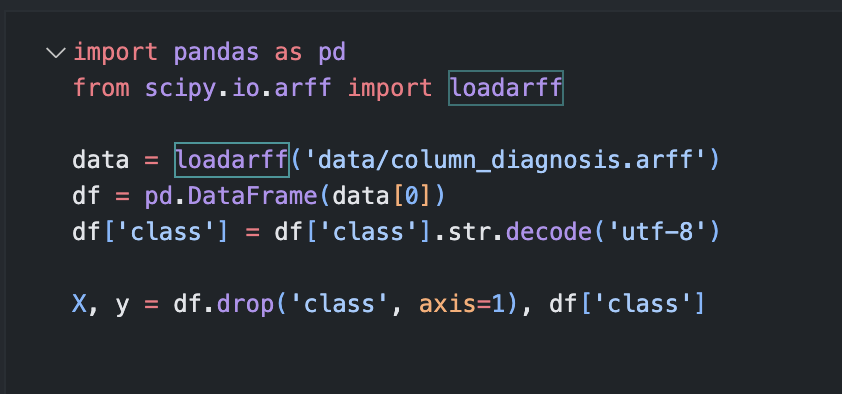
\includegraphics[scale=0.8]{images/code2.png}
\end{center}

\begin{enumerate}[leftmargin=\labelsep]
    \item Compare the performance of $k$NN with $k = 5$ and naïve Bayes with Gaussian assumption
    (consider all remaining parameters for each classifier as sklearn's default):

    \begin{center}
        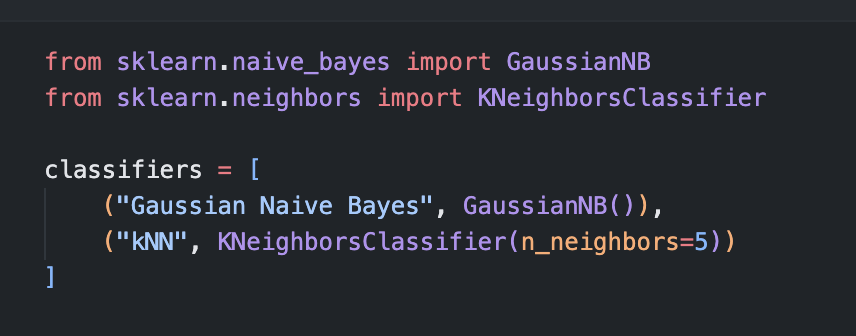
\includegraphics[scale=0.8]{images/code3.png}
    \end{center}

    \begin{enumerate}
        \item Plot two boxplots with the fold accuracies for each classifier.
        
        \begin{center}
            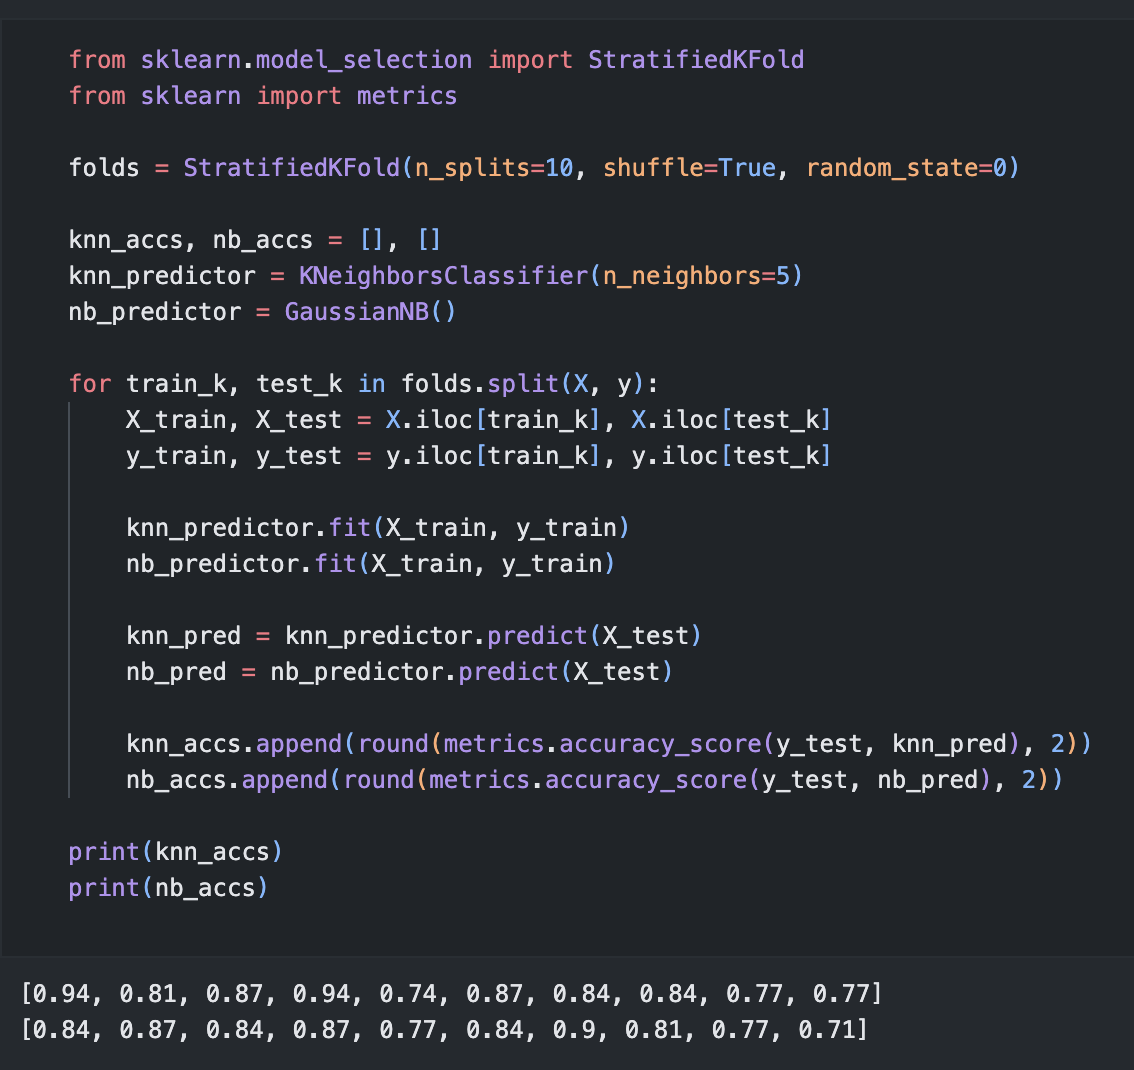
\includegraphics[scale=0.5]{images/code4.png}
        \end{center}

        \begin{center}
            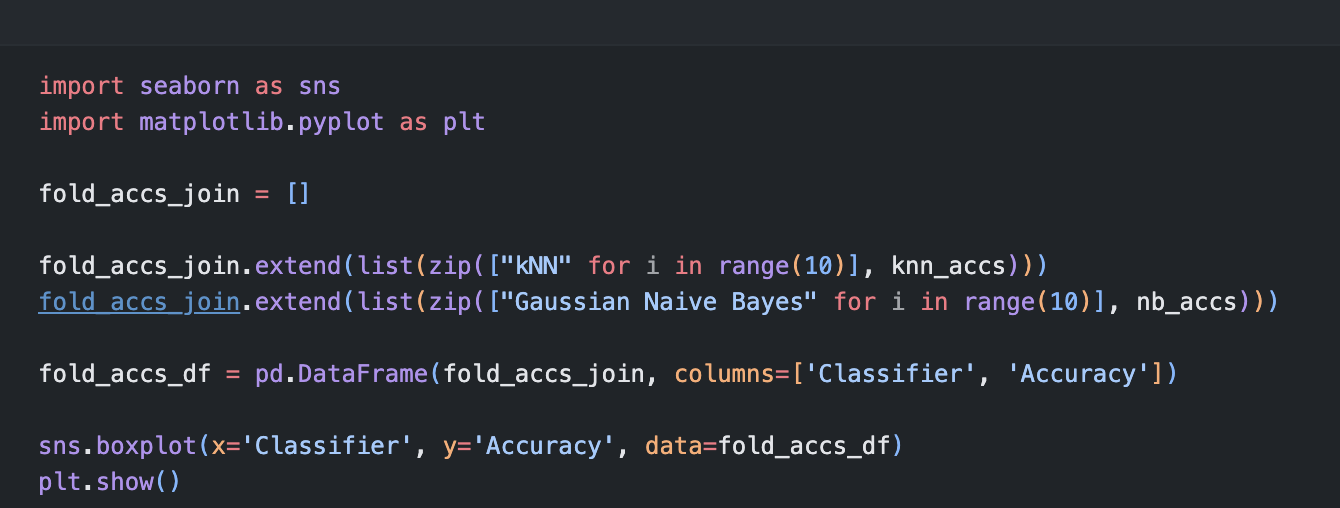
\includegraphics[scale=0.6]{images/code5.png}
        \end{center}

        \vskip 1cm

        Result:

        \begin{center}
            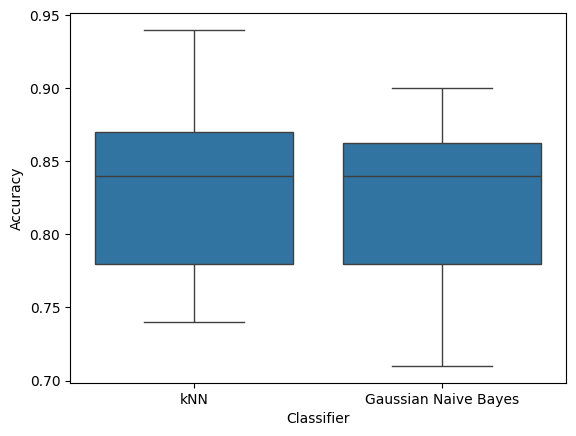
\includegraphics[scale=0.6]{images/graph1.png}
        \end{center}

        \item Using scipy, test the hypothesis “$k$NN is statistically superior to naïve Bayes regarding
        accuracy”, asserting whether is true.

        \begin{center}
            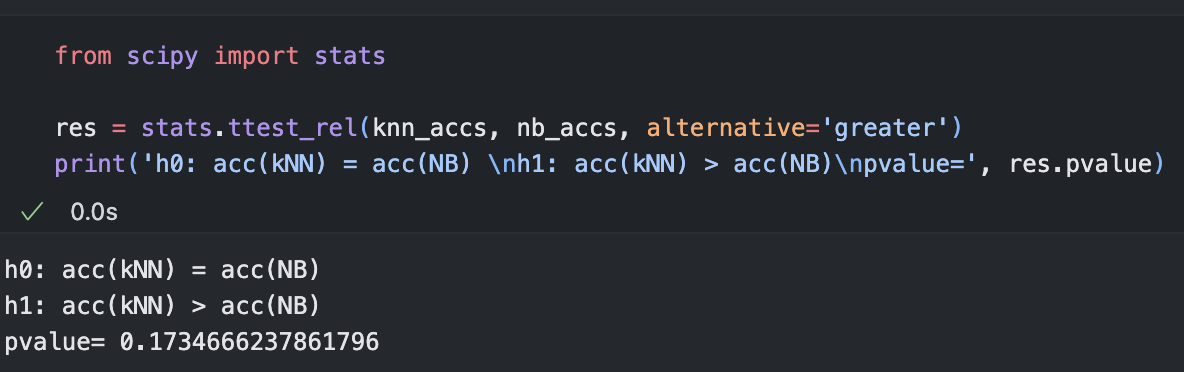
\includegraphics[scale=0.6]{images/code6.png}
        \end{center}

        Visto que o p-value é aproximadamente 0.17, não podemos rejeitar a hipótese nula para os valores de significância usuais (geralmente igual ou inferior a 0.05), a favor da hipótese "kNN is statistically superior to naïve Bayes regarding accuracy".
    \end{enumerate}

    \item Consider two $k$NN predictors with $k = 1$ and $k = 5$ (uniform weights, Euclidean distance,
    all remaining parameters as default). Plot the differences between the two cumulative confusion
    matrices of the predictors. Comment.

    \begin{center}
        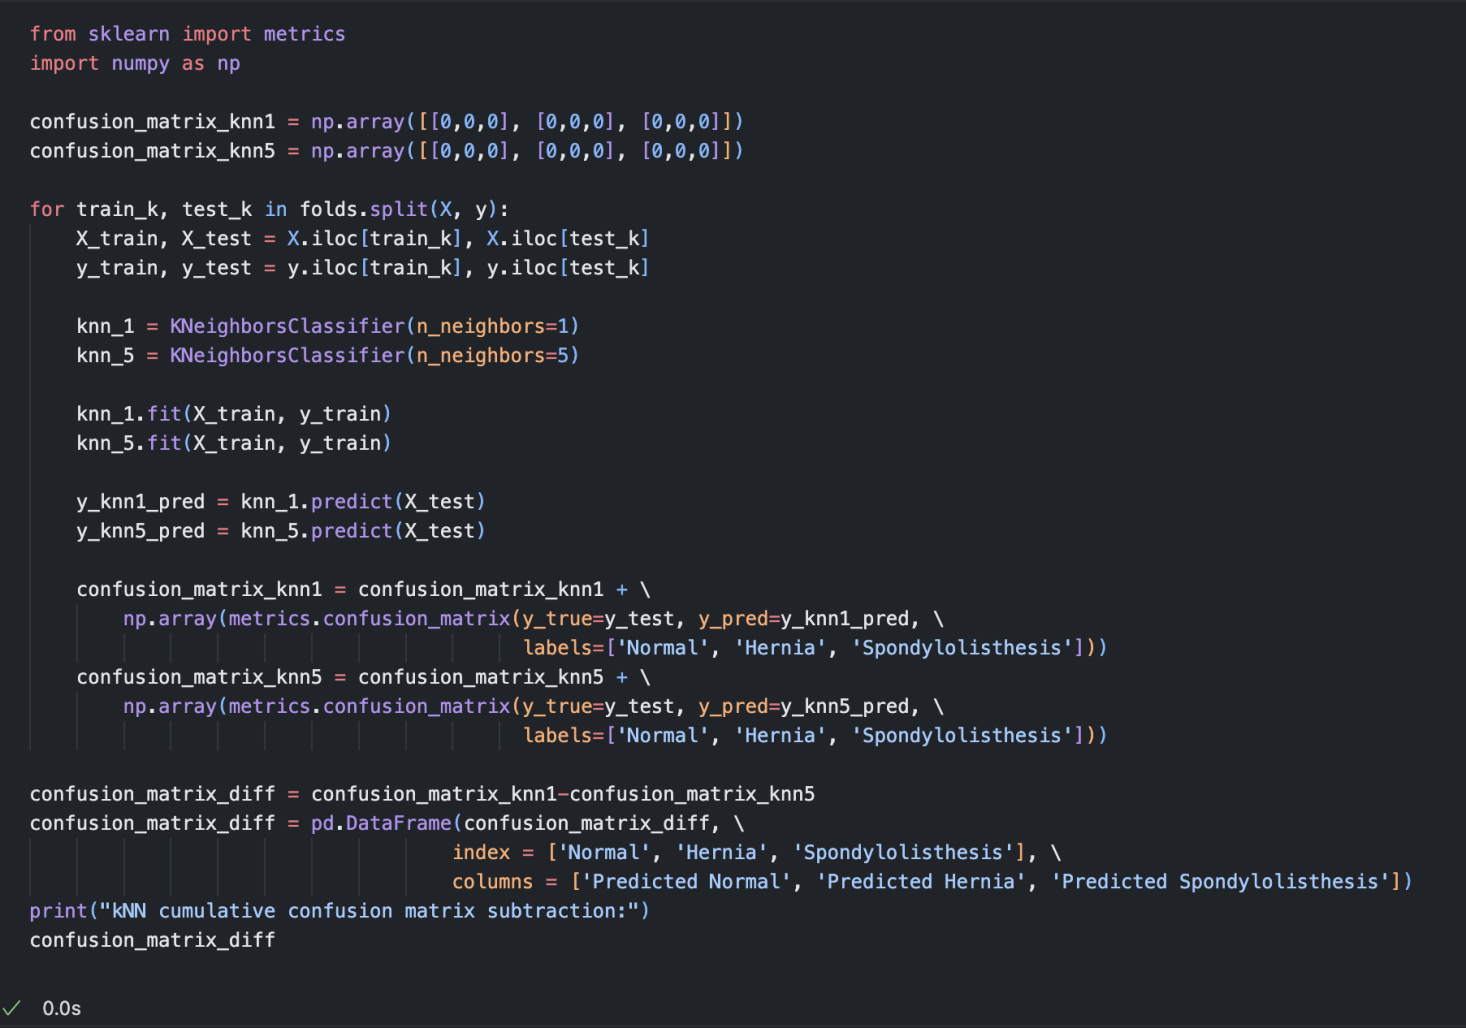
\includegraphics[scale=0.3]{images/code7.png}
    \end{center}

    Result:

    \begin{center}
        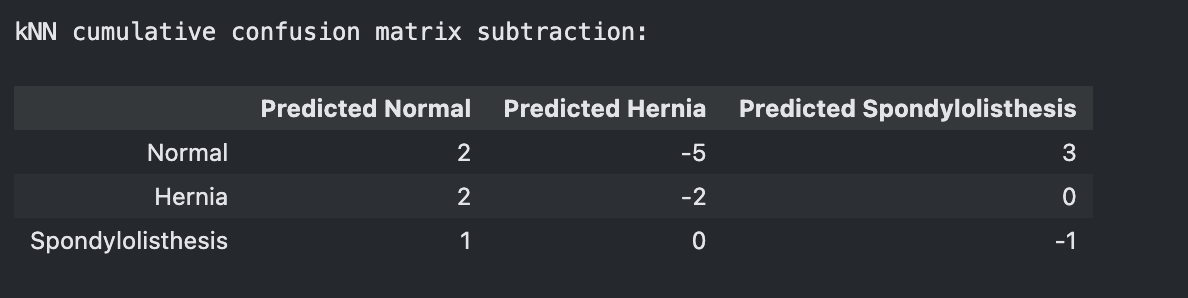
\includegraphics[scale=0.6]{images/table1.png}
    \end{center}

    Ao fazemos a substração das matrizes de confusão cumulativas para o classificador kNN de k=1 com o classificador kNN de k=5, conseguimos concluir que valores negativos na substração indicam um maior número nessa célula a favor do classificador kNN de k=5, e se for positivo, a favor de kNN de k=1.

    Ao observarmos as colunas, conseguimos concluir que o classificador de k=1 tem a tendência de classificar mais casos como "Normal" e que o classificador k=5 tem a tendência de classificar mais casos como "Hernia". Esta tendências podem ser observadas pela errada classifcação de mais 5 casos com "Hernia" enquanto na realidade era "Normal" pelo classificador k=5, enquanto que o classificador k=1 classificou erradamente como "Normal" duas observações "Hernia" e 1 observação "Spondylolisthesis". Curiosamente, ambos os modelos classificaram o mesmo número de casos reais de "Spondylolisthesis" como "Hernia".
    
    No caso da classe "Spondylolisthesis" os classificadores possuem uma tendência semelhante ao classificar observações para esta classe enquanto se trata de uma "Hernia". Por outro lado, o classificador k=1 preveu mais 3 observações com esta classe que eram "Normal" do que o classificador k=5, enquanto que o classificador k=5 classificou corretamente uma observação a mais do que k=1 para esta classe.
    
    Para classificações corretas (True Positives), o classificador k=5 classifica mais observações corretamente que se tratam de "Hernia" e "Spondylolisthesis", enquanto que k=1 classifica corretamente mais observações do tipo "Normal". No entanto, no geral, o classificador k=5 possui uma accuracy maior.
    
    Conseguimos então concluir que o kNN de k=5 possui uma maior recall para "Hernia". Isto é importante para o caso em estudo, visto que estamos a testar condições médicas e por isso um false positive é melhor do que um false negative. Isto, aliado ao facto de não haverem diferenças muito significativas para a deteção de "Spondylolisthesis", faz nos parecer que o classificador k=5 é mais adequado ao diagnóstico médico.
    \item Considering the unique properties of column\_diagnosis, identify three possible difficulties
    of naïve Bayes when learning from the given dataset.

    Ao utilizarmos naïve Bayes, estamos a assumir independência entre as variáveis de input, o que poderá causar perda de informação se existir dependências entre elas. Neste caso, para um diagnóstico de coluna, geralmente é necessário considerar vários pontos (variáveis de input) relacionados, para se poder classificar corretamente, ou seja, neste caso perde-se informção ao usar este modelo. Este facto, junto com a assumção gaussiana, faz com que haja perda de informação, visto que o mais correto seria considerar as variáveis de imput como uma gaussiana multivariada.

    Para além disso, para utilizar este modelo, apenas usámos uma amostra de 310 observações, ou seja um número limitado de observações da população inteira, o que pode gerar resultados não descritivos da população que estamos a estudar, ainda por cima considerando a dimensionalidade do conjunto de dados.

    Para estes dados, também falta balançeamento de classes, visto que existe 150 observações de "Spondylolisthesis", 100 observações de "Normal" e 60 observações de "Hernia" (obtidos através da função df.value\_counts("class")). Ou seja, visto que o sklearn.naive\_bayes utiliza um critério MAP, é criado bias através dos priors.

    \begin{center}
        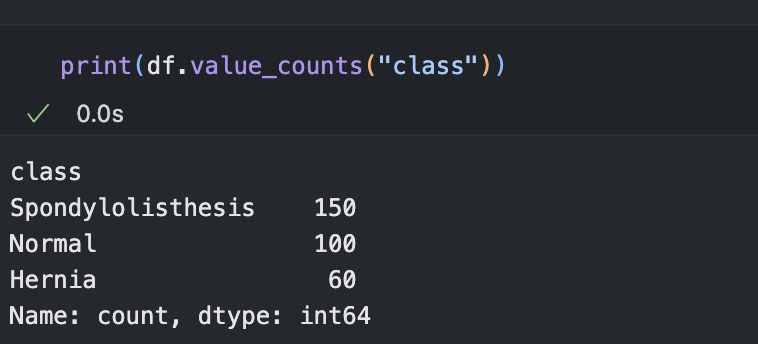
\includegraphics[scale=0.6]{images/code8.png}
    \end{center}
\end{enumerate}


\end{document}
